\documentclass[a4wide,12pt]{article}

\usepackage{verbatim}
\usepackage{listings}
\usepackage{graphicx}
\usepackage{a4wide}
\usepackage{color}
\usepackage{amsmath}
\usepackage{amssymb}
\usepackage[T1]{fontenc}
\usepackage{cite} % [2,3,4] --> [2--4]
\usepackage{shadow}
\usepackage{hyperref}
\usepackage{algorithm2e}
\usepackage{ae}

\begin{document}
\begin{titlepage}
\begin{center}
\vspace*{5cm}
\Large\textbf{FYS4150 - computational physics}
\vspace{1cm}

\Large\textbf{Project 5}
\vspace*{1cm}

\large\textbf{Diffusion in one and two dimensions}
\vspace{1cm}

\large\textit{Candidate number: 109}


\textit{Cooperated with candidate number: 11 and 6}
\end{center}
\end{titlepage}


\section*{Abstract}
We have in this exercise solved the diffusion equation for both one and two dimensions
with different numerical methods.
The random walk method worked nice in 1 dimension, but for 2 dimensions we only got a one dimensional
projection of what should be a two dimensional result. 
The implicit and explicit methods worked nicely, but have not the 
We arrived at the conclusion that the best way to solve the two dimensional 
diffusion equation is by the implicit Jacobi method
We will see that the random walk models are best for solving the neurotransmitters as these have
the right initial and boundary conditions incorporated. 

\section*{Introduction}
Inside nerve cells, there are synaptic vesicles containing neurotransmitter molecules. 
When an action potential in the cell is initiated, synapticle vesicles release 
neurotransmitters through the cell membrane, into a gap called a synaptic cleft, 
and make their way into another cell. 
This is how signals are transferred between nerve cells.

In this project we will model neurotransmitter molecules diffusing from the presynaptic membrnae of a synaptic cleft
to the postsynaptic. This we will do by solving the diffusion equation by the random walk method in one and two dimension. 
Further I will
solve the 2D diffusion equation by the explicit Forward Euler scheme and the implicit Jacobi scheme. 
We will see the difference between having a constant step length and a random step length for the solution by 
Monte Carlo in one dimension. For the explicit and implicit two dimensional scheme we will also do a short discussion on the stability of the methods and their precision. 


To solve the exercises in this project we have used the codes you can find in this 
\href{https://www.dropbox.com/sh/82caiwdrs1i5a8c/mkOkvTWc-I}{dropbox folder}\footnote{https://www.dropbox.com/sh/82caiwdrs1i5a8c/mkOkvTWc-I}. I do not include any code in this report as the Dropbox folder is anonymous.  
The different programs called main().cpp are programs where we set initial conditions, time step and different values needed in the solver. The solvers for the Monte Carlo method
can be found in Walker.cpp and lastly CPhys.cpp contains the method for the implicit and the explicit scheme. 
CPhys.cpp is a program package we have created ourselves, this package contains many other methods and classes and the source code is therefore longer than just what we have done in this project. 

We have throughout this project used 10000 walkers when using the Monte Carlo method even in two dimensions to save time usage.  
I have placed all the plots at the end of the report to gain a more readable report. 
We have plotted all the five different schemes for three different end times 0.01, 0.1 and 0.5. 
\section*{Methods}
The first thing we were asked to do was to make a program that would solve the one dimensional diffusion equation 
\[
\frac{\partial^{2}u(x,t)}{\partial x^{2}} = \frac{\partial{u(x,t)}}{\partial t}
\]
\[
u(x,0)= 0 \hspace{0.5cm} 0 < x < 1
\]
\[
u(0,t)= 1 \hspace{0.5cm} t > 0
\]
\[
u(1,t)= 0 \hspace{0.5cm} t > 0
\]

with the Monte Carlo random walk method. We see that there is a mathematical correlation between random walk and diffusion equation,
by defining a grid
\[
x_{j} = x_{0} + j \Delta x
t_{n} = t_{0} + n \Delta t
\]
where $\Delta x$ is the random walk step size. We can define $P^{n}_{j}$ that a walker is at point j at time step n.
This probability is related to the neighbouring points
\[
P^{n}_{j} = \frac{1}{2}(P^{n-1}_{j+1}+P^{n-1}_{j-1})
\]
if there is an equal probability for moving to the left or right. By using $P = u\Delta x$ where u is the probability density
we find
\[
u^{n}_{j} = \frac{1}{2}(u^{n-1}_{j+1}+u^{n-1}_{j-1})
\]
\[
\frac{u^{n}_{j} - u^{n-1}_{j}}{\Delta t} = \frac{\Delta x^{2}}{2\Delta t}\frac{u^{n-1}_{j+1}-2 u^{n-1}_ {j}+u^{n-1}_{j-1}}{\Delta x^{2}}
\]
We know get for $\Delta x, \Delta t \rightarrow 0$ and $D = \frac{\Delta x^{2}}{2\Delta t}$ we get
\[
 D\frac{\partial^{2}u(x,t)}{\partial x^{2}} = \frac{\partial u(x,t)}{\partial t}
\]
which we recognise as the diffusion equation.

The algorithm we used for the Monte Carlo method was 
\begin{enumerate}
\item{Decide the number of walkers, number of steps and $\Delta t$}
\item{Itterate over the number of steps and walkers}
\item{Use a random number to finad what way the walker moves}
\item{collect the data}
\end{enumerate}

\begin{algorithm}[H]
\SetAlgoLined
\For{ step = 0 ; step*dt < T ; step++}{
\For{walker in walkers}{
\If{pos < minPos || pos > maxPos} {continue}
\If{left} {pos += l} 
\If{right} {pos -= l}

posArray[step] += pos 

pos2Array[step] += pos*pos 

probArray[pos] += 1
	}
}
\end{algorithm}
The implementation of this you can see in mainWalker.cpp and Walker.cpp. The analytic solution for this one dimensional case we found in the last project so I will only give the result.
\[
u(x,t) = 1 - x - \frac{2}{\pi}\sum\limits_{n=1}^{\infty} \frac{1}{n} e^{-n^{2}\pi^{2}t} sin(n\pi x)
\]
which we will compare to our numerical solutions later. 

We have been given the step length $l = \sqrt{2*D*\Delta t}$ which we will use in the beginning of the one dimensional case
before we start using a random step length $l = \sqrt{2*D*\Delta t}\eta$ where $\eta$ is taken from a normal distribution.


For the two dimensional case we have to find new initial and boundary conditions, the Monte Carlo method will converge towards the same no matter how we
implement the new conditions. They are however needed for the explicit and implicit schemes we discuss later. 
After scouring the lecture notes and internet for clues we found the project from last year where we found the following conditions:
Initial conditions
\[
u(x,y,0)=(1-y)\exp{(x)}  \hspace{0.5cm} 0 \le x, y \le 1
\]
and for the boundary conditions (so-called Dirichlet conditions) we found
\[
u(0,y,t)= (1-y)\exp{(t)} \hspace{0.5cm} t \ge 0 \hspace{0.5cm} 0\le y \le 1,
\]
\[
u(1,y,t)= (1-y)\exp{(1+t)} \hspace{0.5cm} t \ge 0 \hspace{0.5cm} 0\le y \le 1,
\]
\[
u(x,0,t)= \exp{(x+t)} \hspace{0.5cm} t \ge 0 \hspace{0.5cm} 0\le x \le 1,
\]
and
\[
u(x,1,t)= 0 \hspace{0.5cm} t \ge 0 \hspace{0.5cm} 0\le x \le 1.
\]

Which gives the following closed form solution 
\[
u(x,t) = (1-y)e^{x+t}.
\]

It may be worth pointing out that these boundary conditions do not relate to the boundary conditions from before. The only connection is that $x, y \in [0,1]$ is still valid. 
The algorithm used for solving the two dimensional solution with the Monte Carlo method, which can also be found in Walker.cpp. 

\begin{algorithm}[H]
 \SetAlgoLined
\For {step = 0 ; step*dt < T ; step++}{
	\For {walker in walkers} {
\If{posX < minPosX || posX > maxPosX} {continue} 
\If{posY < minPosY || posY > maxPosY} {continue}
\If{up} {posY += l}
\If{down} {posY -= l} 
\If{left} {posX += l} 
\If{right} {posX -= l}

posArrayX[step] += posX 

posArrayY[step] += posY 

pos2ArrayX[step] += posX*posX 

pos2ArrayY[step] += posY*posX 

probArrayX[posX] += 1 

probArrayY[posY] += 1
		}
	}
\end{algorithm}

We wanted to create a matrix instead of two arrays for the probability, but unfortunately it took too much time 
to time to get proper results from this. So the two dimensional walker case does not look like the implicit, the explicit or the analytic solution. 

Our next important task is to implement the two dimensional Euler scheme for the diffusion equation. The way to do this is pretty easy
the formula for doing this is:
\[
u(x,y,t+\Delta t) = u(x,y,t) + \alpha(u(x+\Delta x,y,t)+u(x-\Delta x,y,t)+u(x,y+\Delta y,t)+u(x,y-\Delta y,t)-4u(x,y,t))
\]
We do this by constructing a matrix for x and y which changes with time and updating and always keeping the boundary conditions the same. 
For the full way we do this you can check in the files mainExplicit2D.cpp and Cphys.cpp in the Dropbox folder. 

Then we go on to solve the diffusion by the two dimensional implicit Jacobi method. The equation we are supposed to use for this task:
\[
u(x,y,t) = \frac{1}{1+4\alpha}(\alpha(u(x+\Delta x,y,t)+u(x-\Delta x,y,t)+u(x,y+\Delta y,t)+u(x,y-\Delta y,t))+u(x,y,t-\Delta t))
\]
Jacobi's algorithm goes as follows
\begin{enumerate}
\item{Make an initial guess for u(x,y) at all interior points (x,y)}
\item{Use the above equation to compute $u^{m}$ at all interior points. The index m stands for iteration number m.}
\item{Stop if prescribed convergence threshold is reached, otherwise continue to the next step.}
\item{Update the new value of u for the given iteration}
\item{Go to step 2}
\end{enumerate}

We still have the same initial and boundary conditions, and the code is in the programs CPhys.cpp and mainImplicit.cpp. 

\section*{Results}

We see from ~\ref{fig:01} that the Monte Carlo solver is pretty close to the analytical solution, and when we plot the differences we get ~\ref{fig:02}.

We then changed to a Gaussian step length  and we got what is seen in figure ~\ref{fig:03} and ~\ref{fig:04}. We see that there is not much difference
between a Gaussian step length and a constant step length when we have as many as 10000 walkers. After we tried to reduce the number of walkers there was still no significant difference between the two different step lengths a seen in ~\ref{fig:06}. 

As already stated we did not get a matrix for the two dimensional walker case, we still got a few nice plots as you can see in ~\ref{fig:07}. We see that the walkers behave equally in the x and y direction, as expected when we have equal probability for each move. Not very much information to draw from this.  

For the explicit and implicit schemes we got some really nice results as you can see in the figures ~\ref{fig:08}, ~\ref{fig:09} and ~\ref{fig:10}. I have now plotted the implicit, explicit and analytic together for the same time step. 
We see that they all behave pretty similarly and should confirm that we have done something right. 
For the Euler we also have to discuss the truncation error and stability criterion, the Euler truncation error is exactly as before
$O(\Delta x^{2},\Delta y^{2},\Delta t)$. 
The stability criterion we can find by assuming a solution on the form $u(x,y,t)=Ae^{i(k_{x}x+k_{y}y-\omega t)}$.
For x we get
\[
\frac{\partial^{2}u(x,y,t)}{\partial x^{2}} = \frac{u(x-\Delta x,y,t)-2u(x,y,t)+u(x-\Delta x,y,t)}{\Delta x^2} =
\]
\[
Ae^{i(k_{x}x+k_{y}y-\omega t)}\frac{e^{i(k_{x}\Delta x)}-2+e^{-i(k_{x}\Delta x}}{\Delta x^2} =
\]
\[
Ae^{i(k_{x}x+k_{y}y-\omega t)}\frac{2(cos(k_{x}\Delta x)-1)}{\Delta x^2} =
\]
\[
Ae^{i(k_{x}x+k_{y}y-\omega t)}\frac{-4(sin^{2}(\frac{k_{x}\Delta x)}{2}}{\Delta x^2}
\]
Similarly for y
\[
\frac{\partial^{2}u(x,y,t)}{\partial y^{2}} = Ae^{i(k_{x}x+k_{y}y-\omega t)}\frac{-4(sin^{2}(\frac{k_{y}\Delta y)}{2}}{\Delta y^2}
\]
For t we get
\[
\frac{\partial u(x,y,t)}{\partial t} = \frac{u(x,y,t+\Delta t)-u(x,y,t)}{\Delta t} = Ae^{i(k_{x}x+k_{y}y-\omega t)}\frac{e^{-i\omega \Delta t}}{\Delta t}
\]
We insert this into the diffusion equation and get
\[
4\alpha(sin^{2}(\frac{k_{x}\Delta x}{2})+sin^{2}(\frac{k_{y}\Delta y}{2})) = 1-e^{-i\omega\Delta t}
\]
We have that $1-e^{-i\omega\Delta t} \le 2$
\[
4\alpha(sin^{2}(\frac{k_{x}\Delta x}{2})+sin^{2}(\frac{k_{y}\Delta y}{2})) \le 2
\]
\[
alpha \le \frac{1}{4\alpha(sin^{2}(\frac{k_{x}\Delta x}{2})+sin^{2}(\frac{k_{y}\Delta y}{2}))}
\]
 
 \[
 alpha \le min(\frac{1}{4\alpha(sin^{2}(\frac{k_{x}\Delta x}{2})+sin^{2}(\frac{k_{y}\Delta y}{2}))})
 \]
 which gives us
 \[
 \alpha \le \frac{1}{4}
 \]
 This result is what we have used in our program, and we tried on plot outside the stability criterion. You can see this in figure ~\ref{fig:11}. We have also tested different alpha values for the implicit scheme ~\ref{fig:12}
 We have also made a few plots of the difference between the numerical, implicit and explicit solutions, which can be seen in figure ~\ref{fig:13} and ~\ref{fig:14}. There is not much difference to talk about at all.
 
We know check which of the non Monte Carlo methods that is best. The Euler is not as stable as Jacobi, so we check the precision. To check the precision
we have taken their difference from the analytic solution taken explicit - implicit so the positive areas in ~\ref{fig:15} indicate where the implicit is better than the explicit.
This result states that the Jacobi implicit method is a slightly better than Euler for this problem. 
\section*{Conclusion}
We have in this project seen that there is a close relation between diffusion and random walks in one dimension. We also saw that when we changed to a Gaussian step length it did not seem like that much changed. 

We moved on to two dimensional diffusion equation and we saw that for random walk solution we did not get very different results for different times. Indicating that it might not be a good way to solve a two dimensional diffusion equation unless we use a lot of walkers. 
The two other solvers should therefore be better for solving this problem as they produce a matrix as output. 

We have seen that the Jacobi method is not only more stable, but also more precise than the Euler scheme although not by much

We have seen that for the physical problem we have that our choice of initial
and boundary conditions make the random walk models better at explaining
the diffusion of neurotransmitters. 
Even though we only got a projection from two to one dimension we did not need to force any conditions on
this model. 


\begin{figure}[p]
 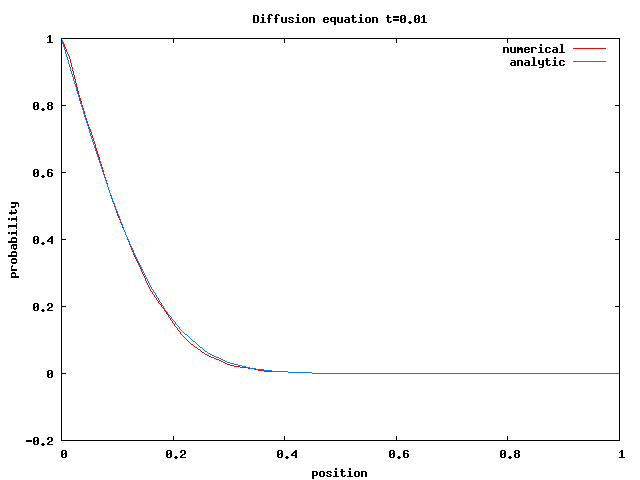
\includegraphics[width=0.5\textwidth]{diff1d001}
 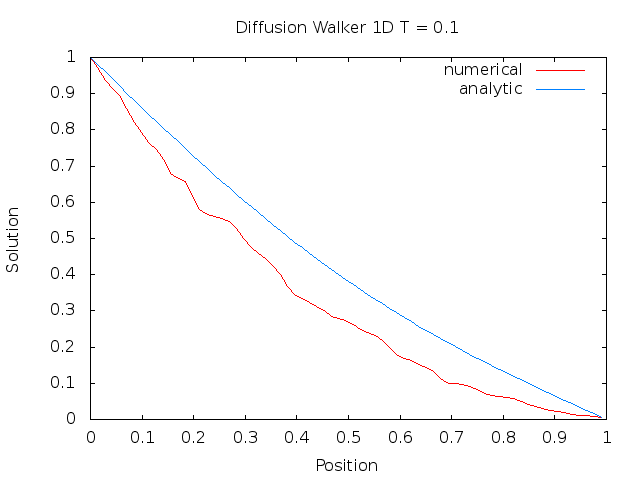
\includegraphics[width=0.5\textwidth]{diff1dt01}
 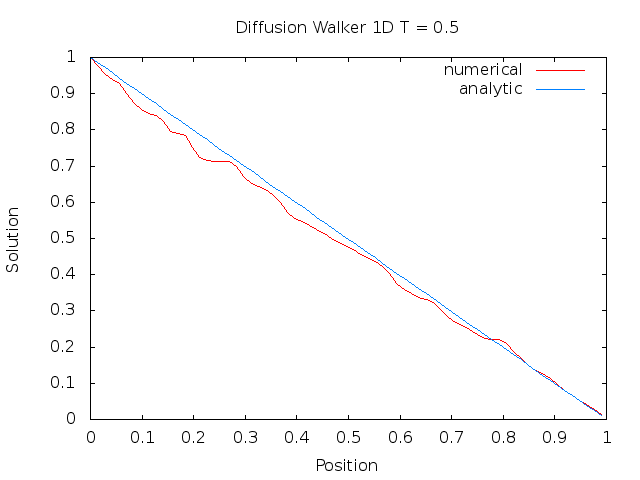
\includegraphics[width=0.5\textwidth]{diff1dt05}
 \caption{1 dimensional Monte Carlo solver and analytic solution for different times}
 \label{fig:01}
\end{figure}

\begin{figure}[p]
 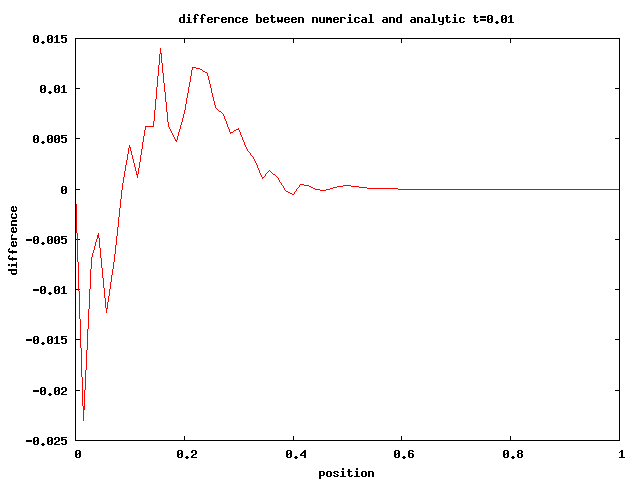
\includegraphics[width=0.5\textwidth]{difference1d001}
 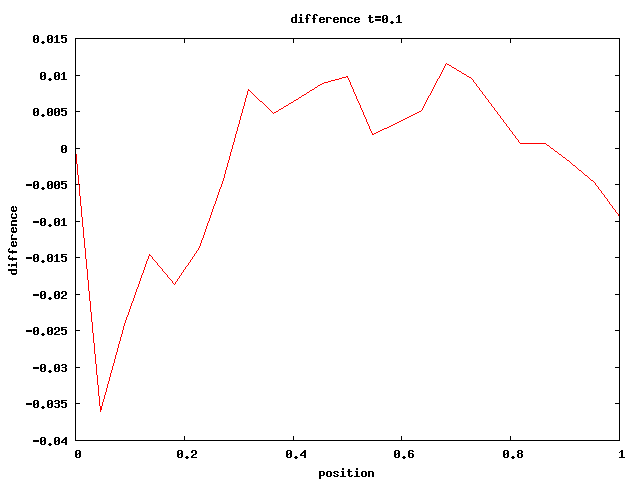
\includegraphics[width=0.5\textwidth]{difference01}
 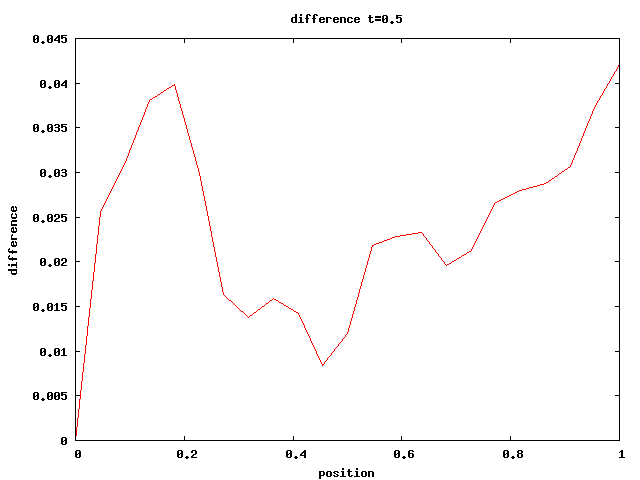
\includegraphics[width=0.5\textwidth]{difference05}walkers as we do. 
 \caption{Difference between analytical and numerical solution for different end times}
 \label{fig:02}
\end{figure}
 
\begin{figure}[p]
 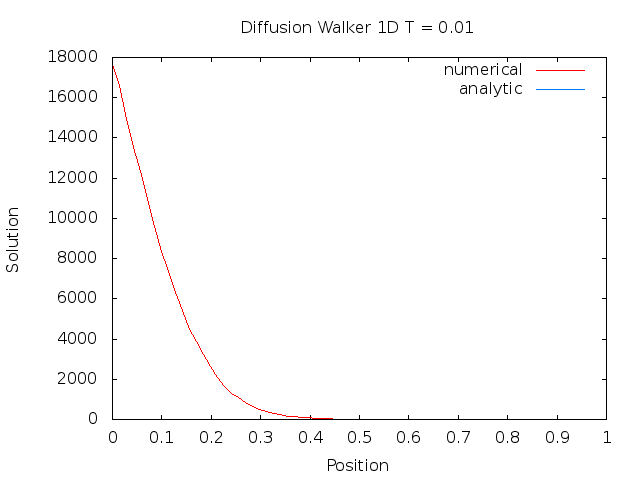
\includegraphics[width=0.5\textwidth]{diff1dt001gauss}
 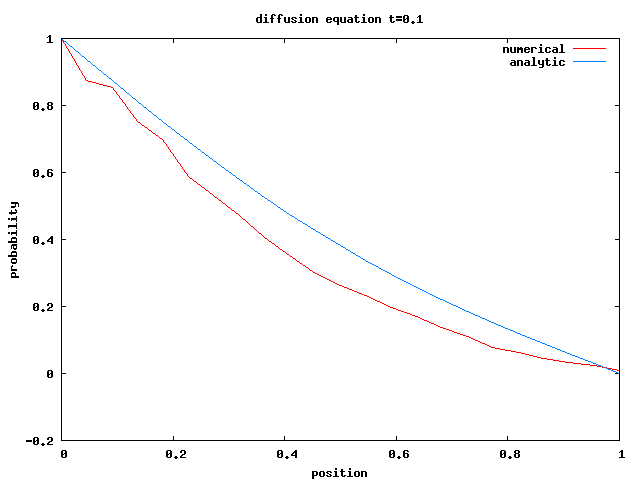
\includegraphics[width=0.5\textwidth]{diff01gauss}
 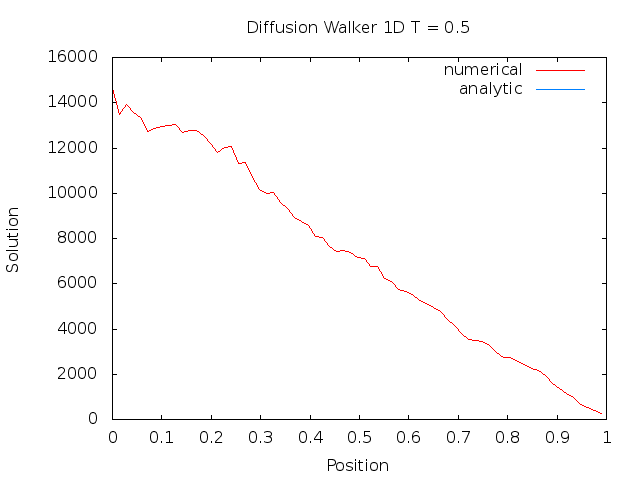
\includegraphics[width=0.5\textwidth]{diff1dt05gauss}
 \caption{1 dimensional Monte Carlo solver and analytic solution for different times with a Gaussian step length}
 \label{fig:03}
\end{figure}
 
\begin{figure}[p]
 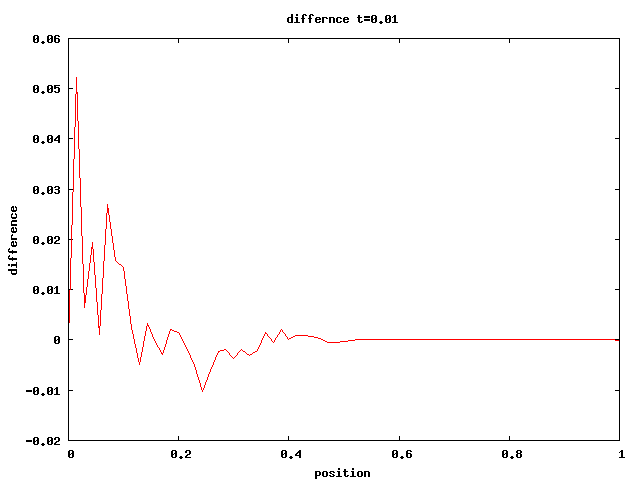
\includegraphics[width=0.5\textwidth]{difference001gauss}
 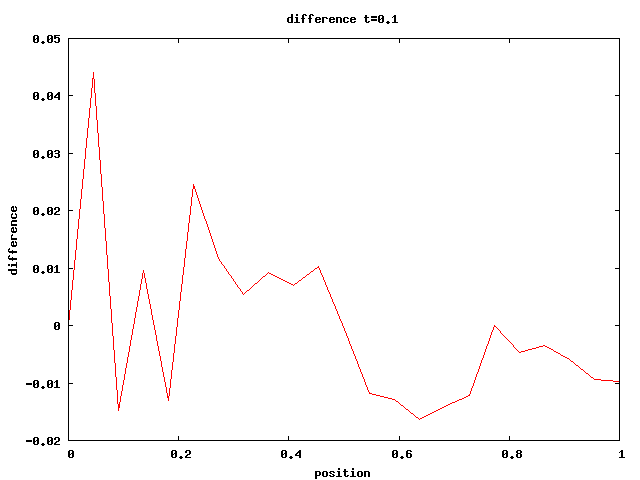
\includegraphics[width=0.5\textwidth]{difference01gauss}
 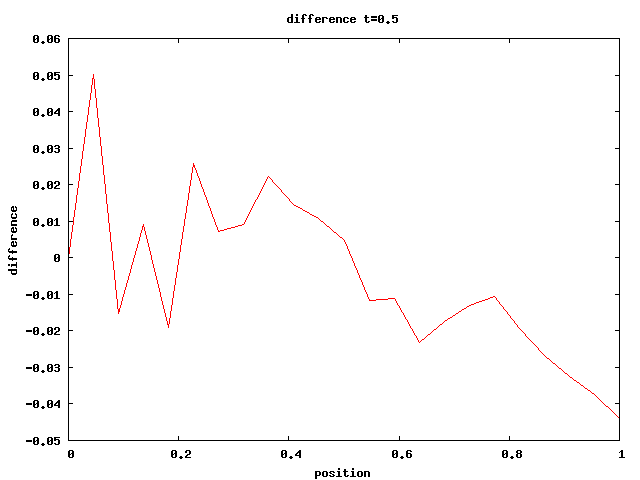
\includegraphics[width=0.5\textwidth]{difference05gauss}
 \caption{Difference between analytical and numerical solution for different end times with a Gaussian step length}
 \label{fig:04}
\end{figure}

\begin{figure}[p]
 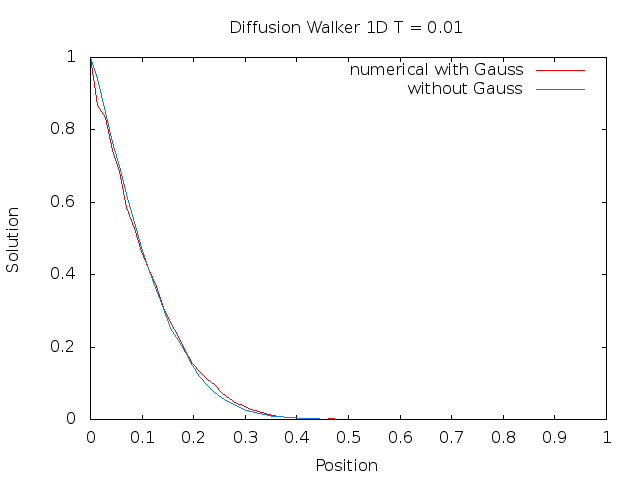
\includegraphics[width=0.5\textwidth]{diff1dt001sm}
 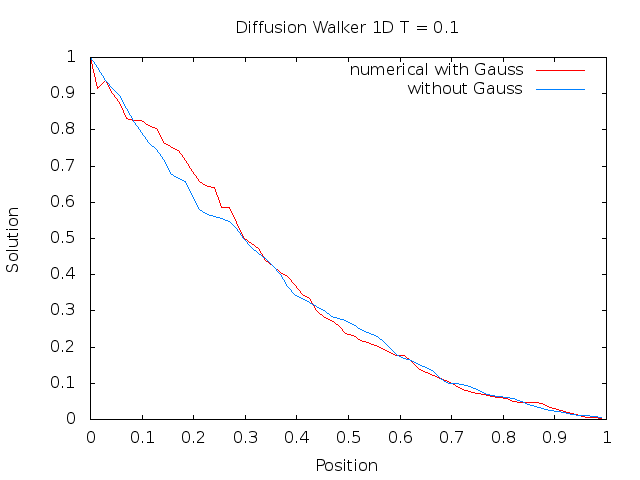
\includegraphics[width=0.5\textwidth]{diff1dt01sm}
 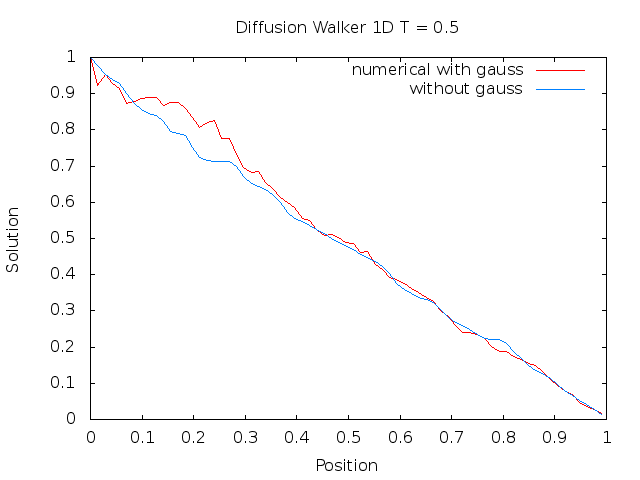
\includegraphics[width=0.5\textwidth]{diff1dt05sm}
 \caption{1 dimensional Monte Carlo solver with both constant step length and Gaussian step length}
 \label{fig:05}
\end{figure}

\begin{figure}[p]
 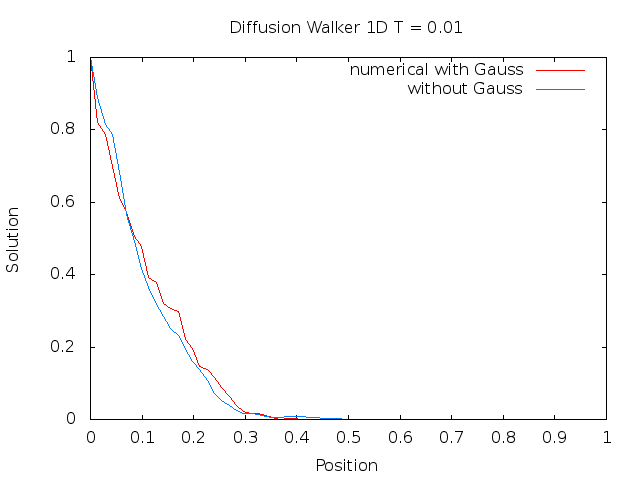
\includegraphics[width=0.5\textwidth]{walk1000}
 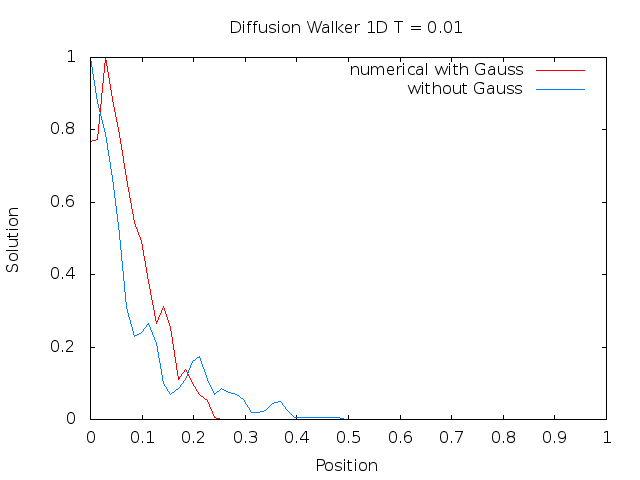
\includegraphics[width=0.5\textwidth]{walk100}
 \caption{1 dimensional Monte Carlo solver with both constant step length and Gaussian step length for 1000 walkers to the left and 100 to the right}
 \label{fig:06}
\end{figure}

\begin{figure}[p]
 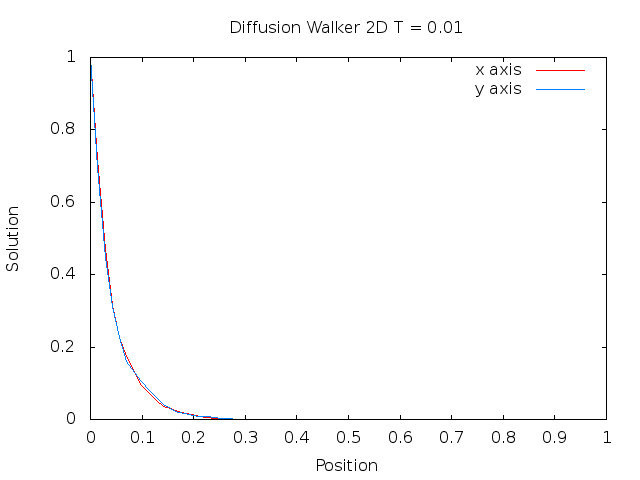
\includegraphics[width=0.5\textwidth]{Walker2DT0_01}
 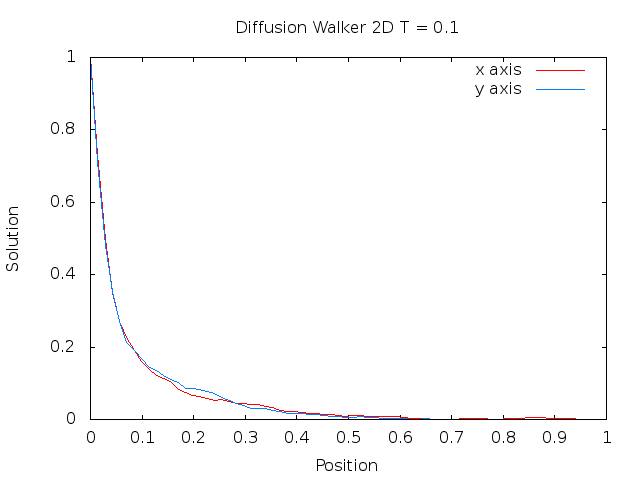
\includegraphics[width=0.5\textwidth]{Walker2DT0_1}
 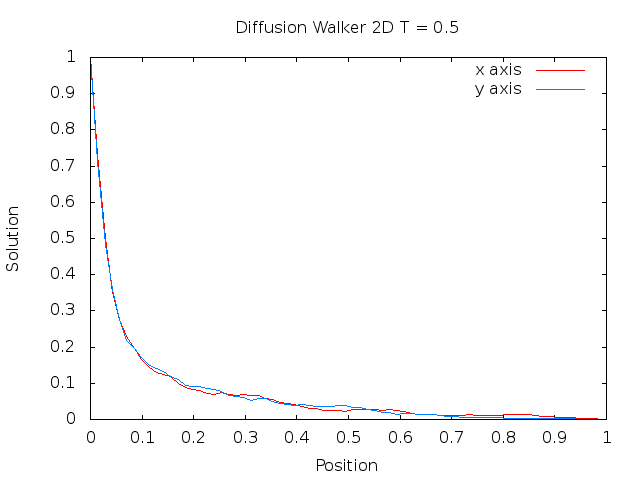
\includegraphics[width=0.5\textwidth]{Walker2DT0_5}
 \caption{2 dimensional Monte Carlo solver with both constant step length for three different step lengths}
 \label{fig:07}
\end{figure}
\begin{figure}[p]
 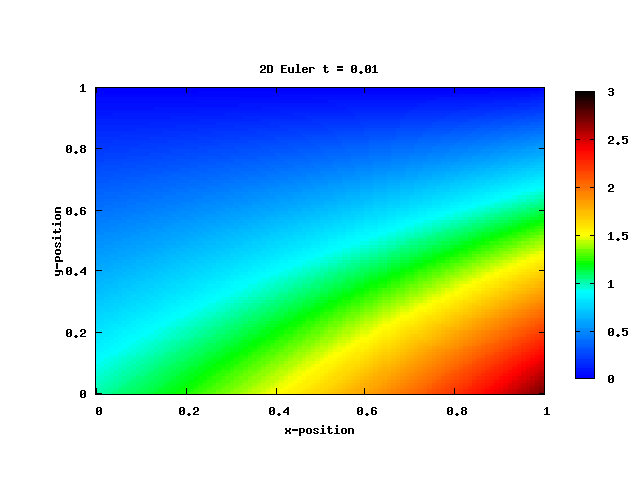
\includegraphics[width=0.5\textwidth]{euler2d001}
 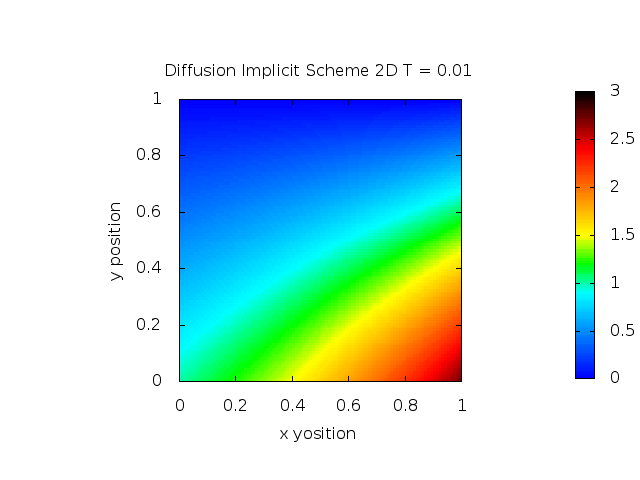
\includegraphics[width=0.5\textwidth]{Implicit2DT0_01}
 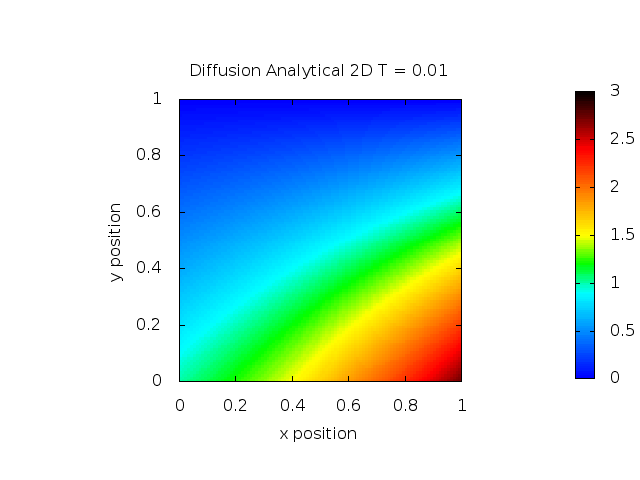
\includegraphics[width=0.5\textwidth]{Analytical2DT0_01}
 \caption{2 dimensional diffusion equation with explicit, implicit and analytical solutions for t=0.01}
 \label{fig:08}
 \end{figure}
 
 \begin{figure}[p]
 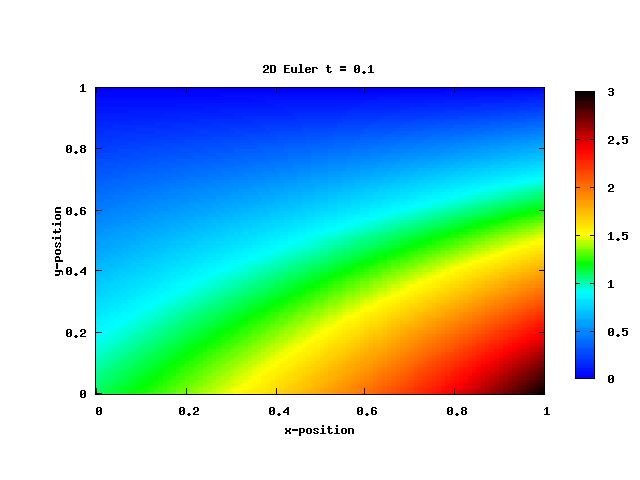
\includegraphics[width=0.5\textwidth]{euler2d01}
 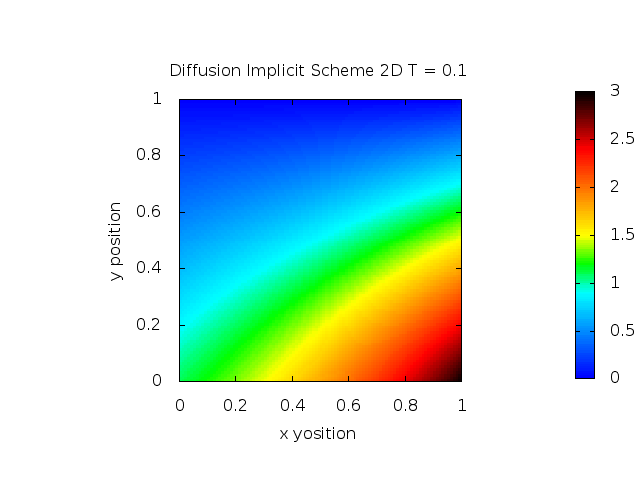
\includegraphics[width=0.5\textwidth]{Implicit2DT0_1}
 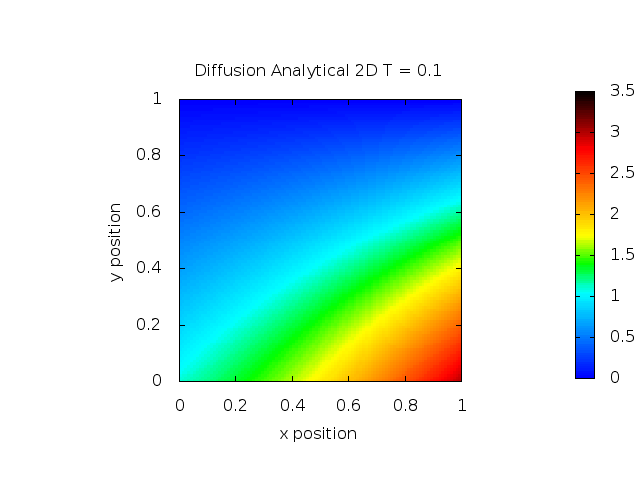
\includegraphics[width=0.5\textwidth]{Analytical2DT0_1}
 \caption{2 dimensional diffusion equation with explicit, implicit and analytical solutions for t=0.1}
 \label{fig:09}
 \end{figure}
 
 \begin{figure}[p]
 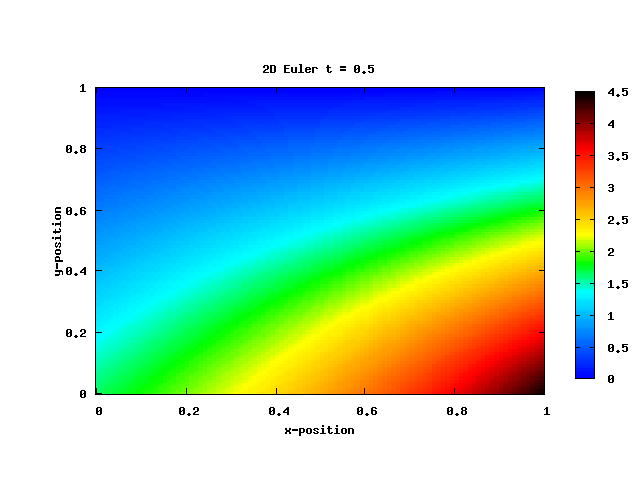
\includegraphics[width=0.5\textwidth]{euler2d05}
 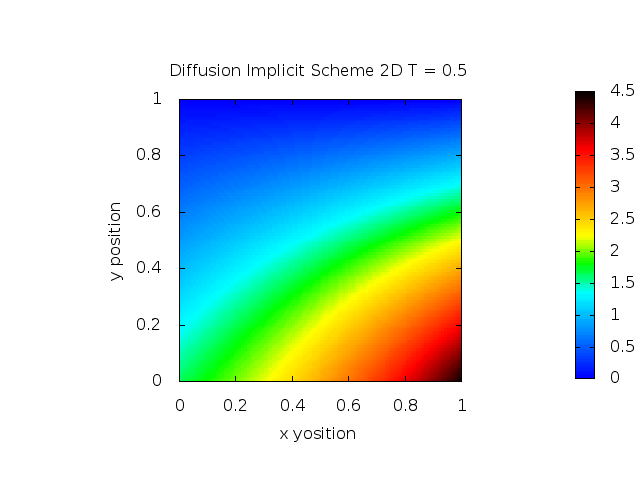
\includegraphics[width=0.5\textwidth]{Implicit2DT0_5}
 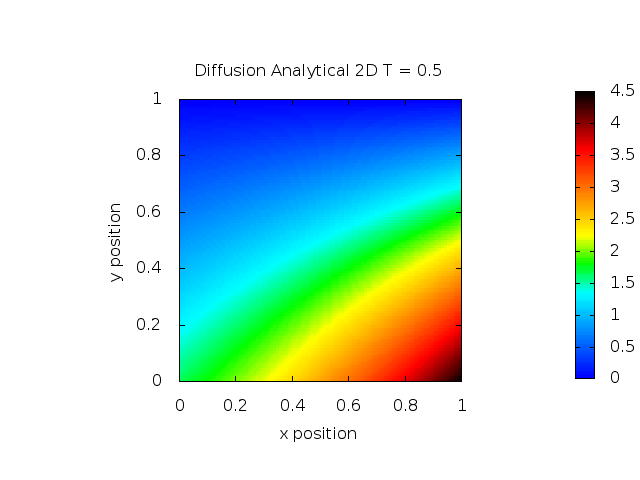
\includegraphics[width=0.5\textwidth]{Analytical2DT0_5}
 \caption{2 dimensional diffusion equation with explicit, implicit and analytical solutions for t=0.5}
 \label{fig:10}
 \end{figure}
 
 \begin{figure}[p]
 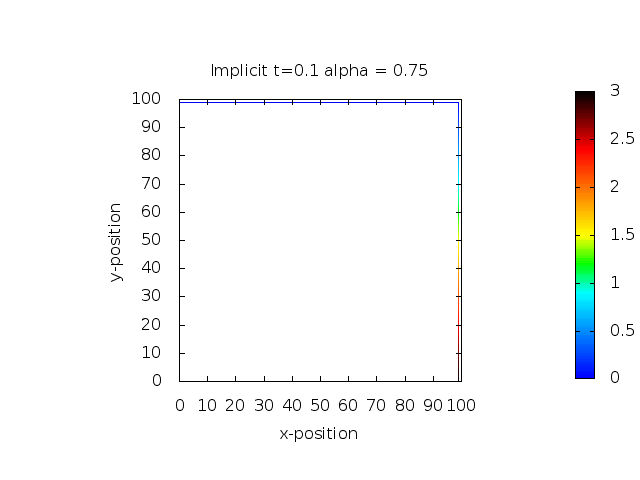
\includegraphics[width=0.5\textwidth]{test3}
 \caption{Plot of explicit with alpha=1, error in the title of the plot}
 \label{fig:11}
 \end{figure}
 
 \begin{figure}[p]
 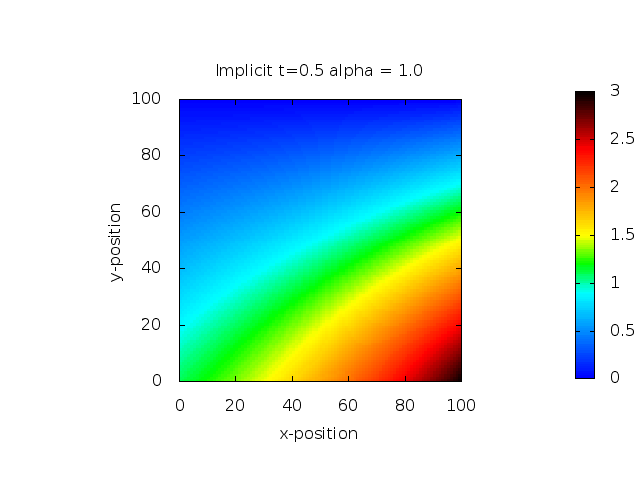
\includegraphics[width=0.5\textwidth]{test}
 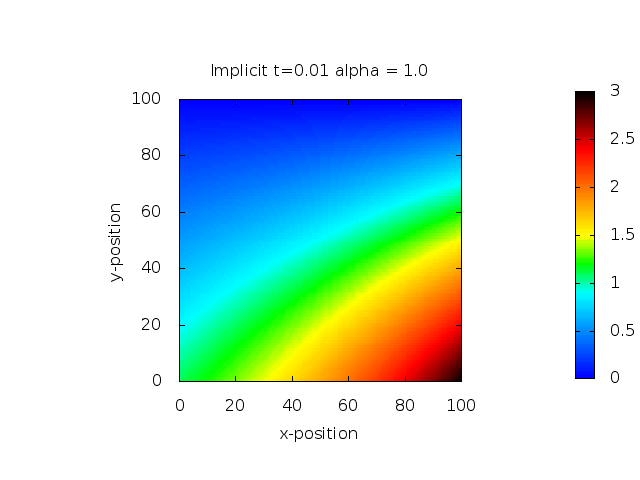
\includegraphics[width=0.5\textwidth]{test2}
 \caption{Plot of implicit for alpha=1.0}
 \label{fig:12}
 \end{figure}
 
 \begin{figure}[p]
 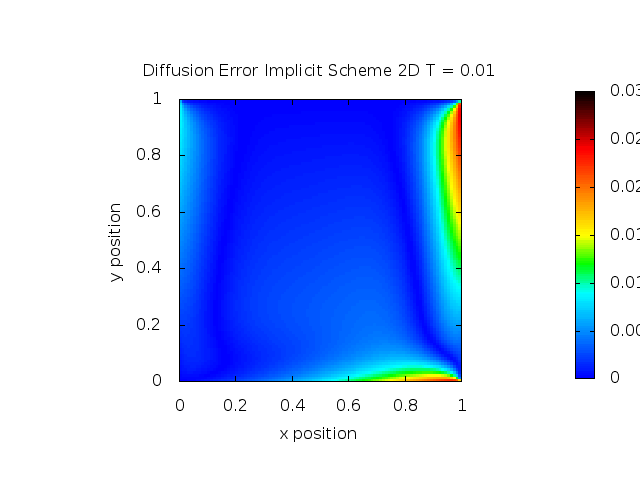
\includegraphics[width=0.5\textwidth]{ErrorImplicit2DT0_01}
 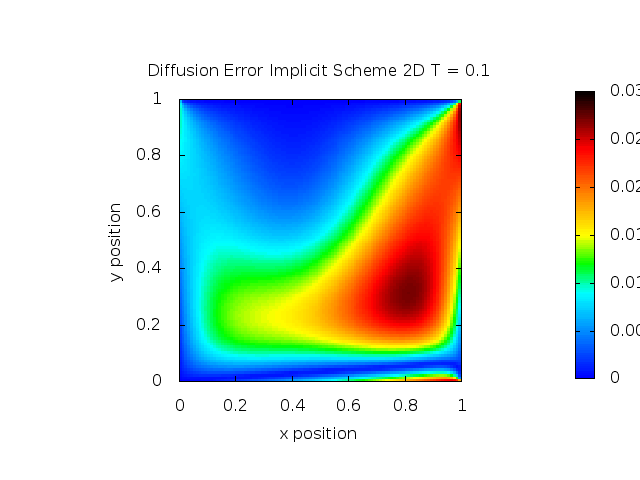
\includegraphics[width=0.5\textwidth]{ErrorImplicit2DT0_1}
 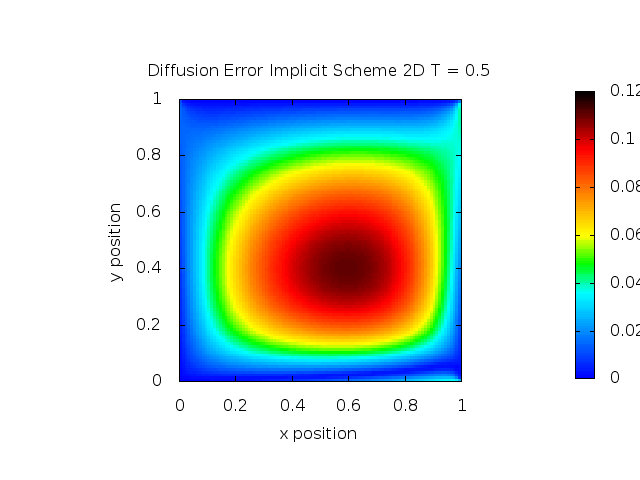
\includegraphics[width=0.5\textwidth]{ErrorImplicit2DT0_5}
 \caption{Difference between the analytical and implicit solution}
 \label{fig:13}
 \end{figure}
 
 \begin{figure}[p]
 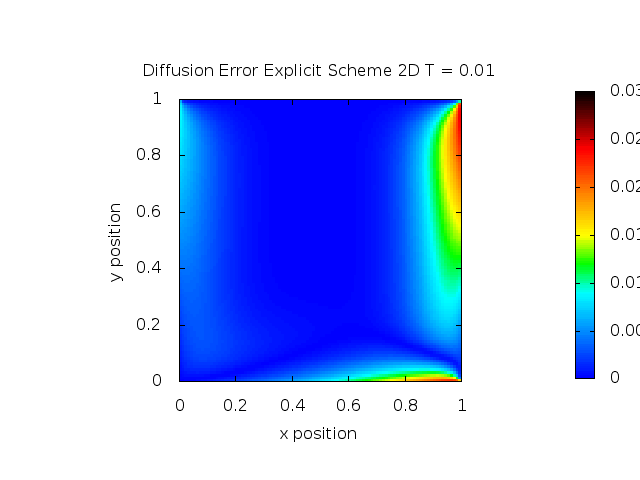
\includegraphics[width=0.5\textwidth]{ErrorExplicit2DT0_01}
 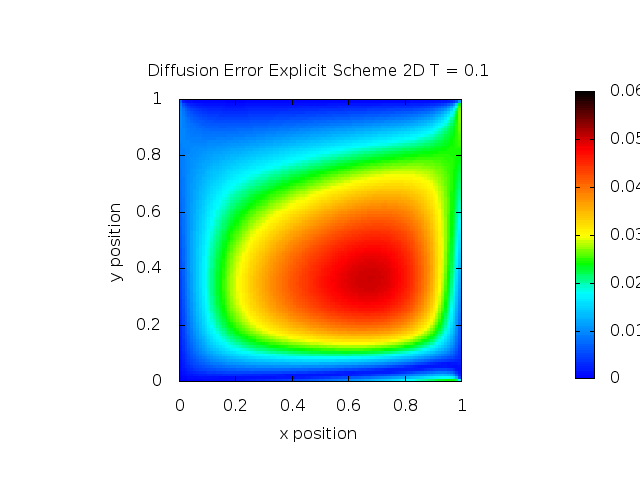
\includegraphics[width=0.5\textwidth]{ErrorExplicit2DT0_1}
 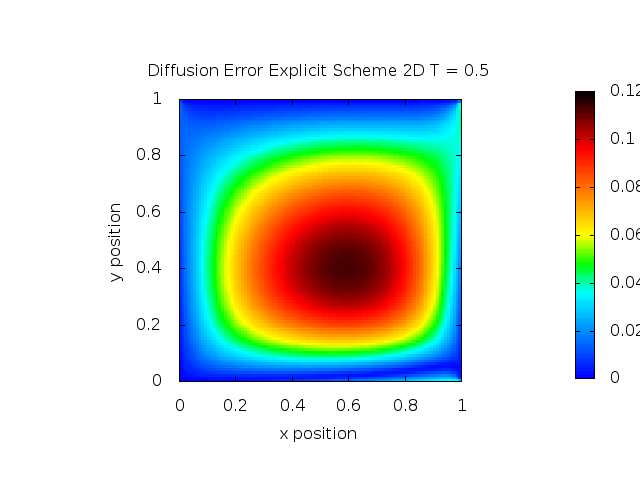
\includegraphics[width=0.5\textwidth]{ErrorExplicit2DT0_5}
 \caption{Difference between the analytical and explicit solution}
 \label{fig:14}
 \end{figure}
 
 \begin{figure}[p]
 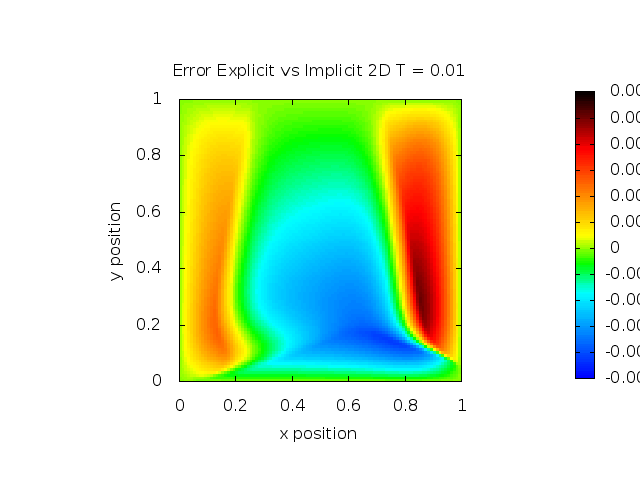
\includegraphics[width=0.5\textwidth]{ErrorExpVsImp2DT0_01}
 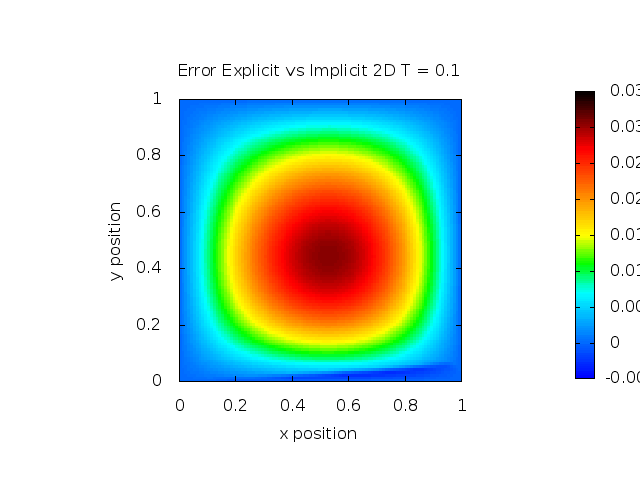
\includegraphics[width=0.5\textwidth]{ErrorExpVsImp2DT0_1}
 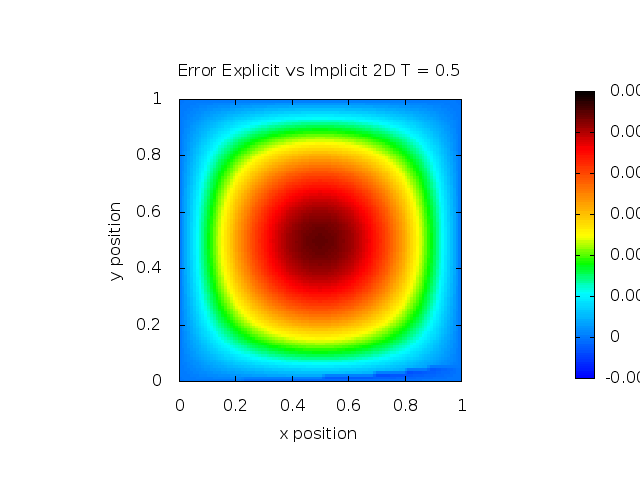
\includegraphics[width=0.5\textwidth]{ErrorExpVsImp2DT0_5}
 \caption{Comparison precision of explicit and implicit}
 \label{fig:15}
 \end{figure}
 
\end{document}